% !TEX root = ../paper.tex

\resizebox{\columnwidth}{!}{
\begin{tikzpicture}
    \node[inner sep=0pt] (original) at (0,0)
        {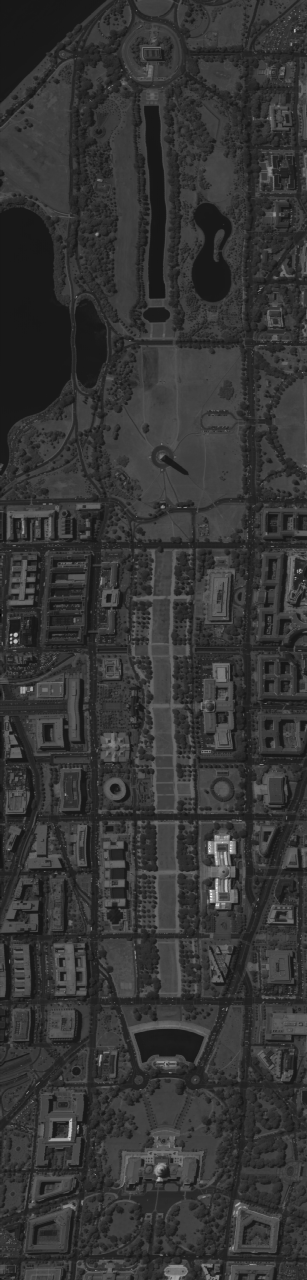
\includegraphics[width=0.8cm,height=3.2cm]{data/DC/0.png}};
        \draw[thick,->] (-0.4,0.8) .. controls (-3,0.8) .. (-3,-0.4);
        \node[inner sep=0pt] (1) at (-3,-2)
            {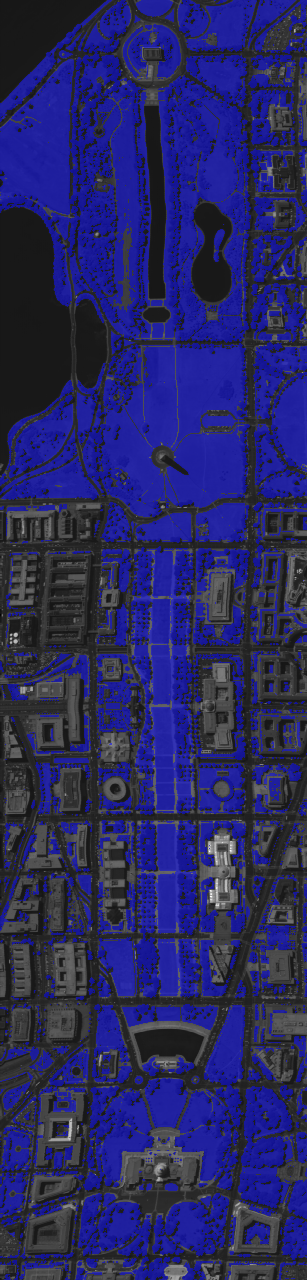
\includegraphics[width=0.8cm,height=3.2cm]{data/DC/1.png}};
            \node[draw, text=orange, fill=white] at (-3,-2) {vegetation};
            \draw[thick,->] (-3.4,-1.2) .. controls (-4.4,-1.2) .. (-4.4,-2.4);
            \node[inner sep=0pt] (3) at (-4.4,-4)
                {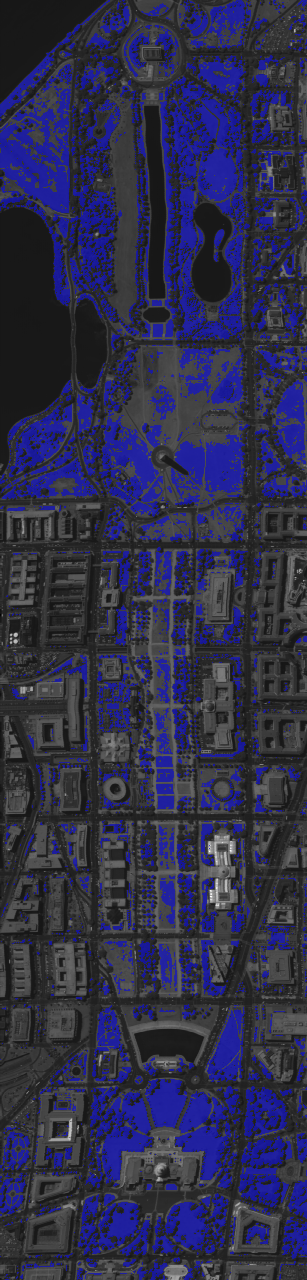
\includegraphics[width=0.8cm,height=3.2cm]{data/DC/4.png}};
                \node[draw, text=orange, fill=white] at (-4.4,-4) {grass};
            \node[below=0.1] at (3.south) {\textbf{3}};
            \draw[thick,->] (-2.6,-1.2) .. controls (-1.6,-1.2) .. (-1.6,-2.4);
            \node[inner sep=0pt] (4) at (-1.6,-4)
                {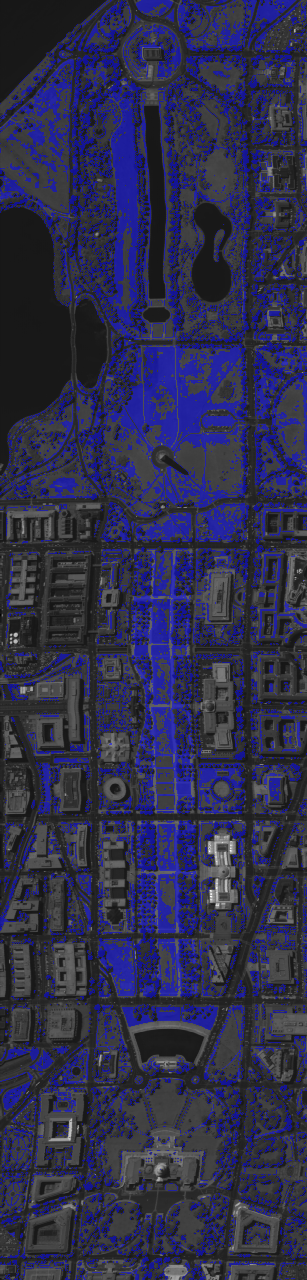
\includegraphics[width=0.8cm,height=3.2cm]{data/DC/3.png}};
                \node[draw, text=orange, fill=white] at (-1.6,-4) {trees};
                \draw[thick,->] (-2,-3.2) .. controls (-2.5,-3.2) .. (-2.5,-4.4);
                \node[inner sep=0pt] (9) at (-2.5,-6)
                    {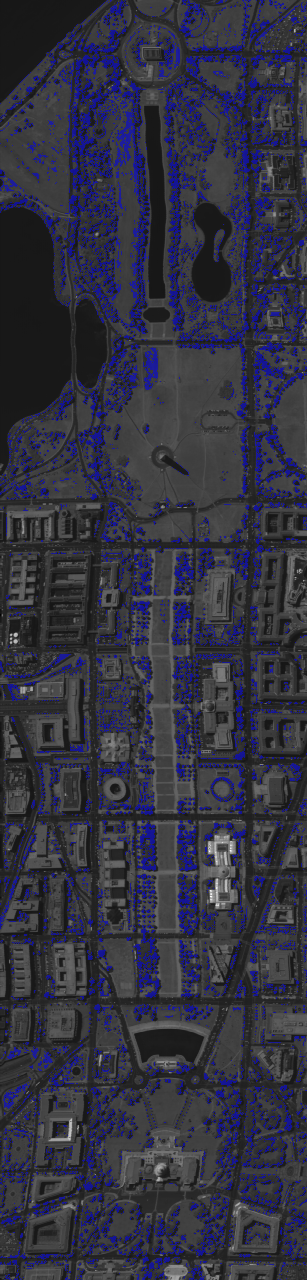
\includegraphics[width=0.8cm,height=3.2cm]{data/DC/7.png}};
                \node[below=0.1] at (9.south) {\textbf{9}};
                \draw[thick,->] (-1.2,-3.2) .. controls (-0.7,-3.2) .. (-0.7,-4.4);
                \node[inner sep=0pt] (10) at (-0.7,-6)
                    {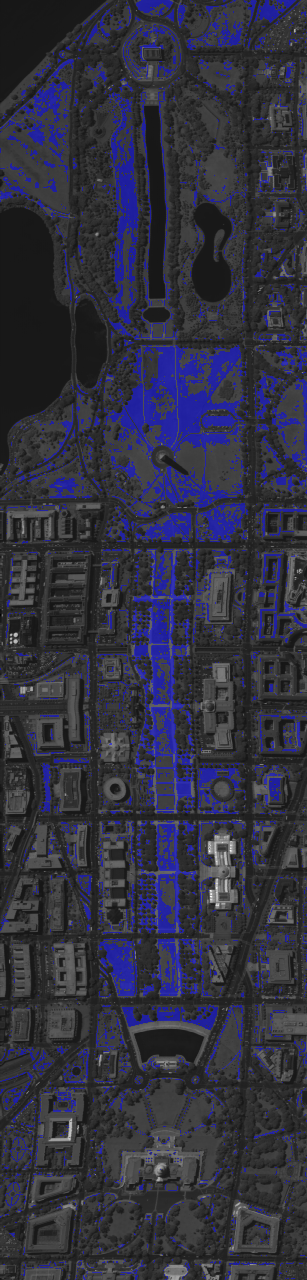
\includegraphics[width=0.8cm,height=3.2cm]{data/DC/8.png}};
                \node[below=0.1] at (10.south) {\textbf{10}};
             \node[below=0.1] at (4.south) {\textbf{4}};
        \node[below=0.1] at (1.south) {\textbf{1}};
        \draw[thick,->] (0.4,0.8) .. controls (3,0.8) .. (3,-0.4);
        \node[inner sep=0pt] (2) at (3,-2)
            {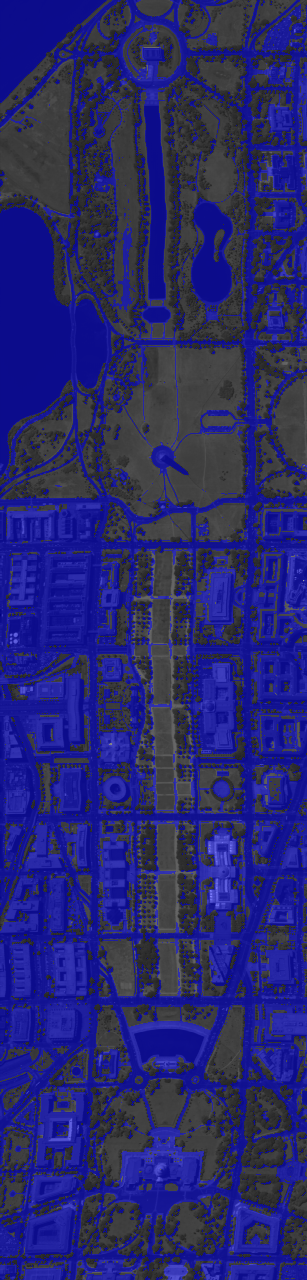
\includegraphics[width=0.8cm,height=3.2cm]{data/DC/2.png}};
            \node[draw, text=orange, fill=white] at (3,-2) {non-vegetation};
            \draw[thick,->] (2.6,-1.2) .. controls (1.6,-1.2) .. (1.6,-2.4);
            \node[inner sep=0pt] (5) at (1.6,-4)
                {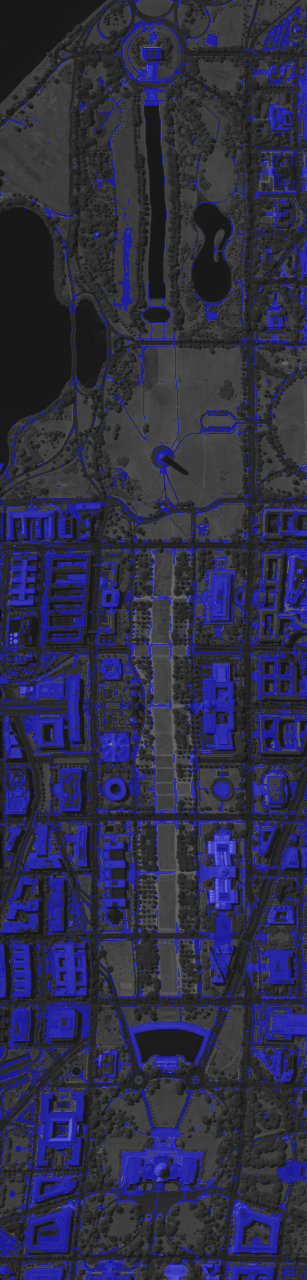
\includegraphics[width=0.8cm,height=3.2cm]{data/DC/6.png}};
                \node[draw, text=orange, fill=white] at (1.6,-4) {buildings};
                \draw[thick,->] (1.2,-3.2) .. controls (0.7,-3.2) .. (0.7,-4.4);
                \node[inner sep=0pt] (11) at (0.7,-6)
                    {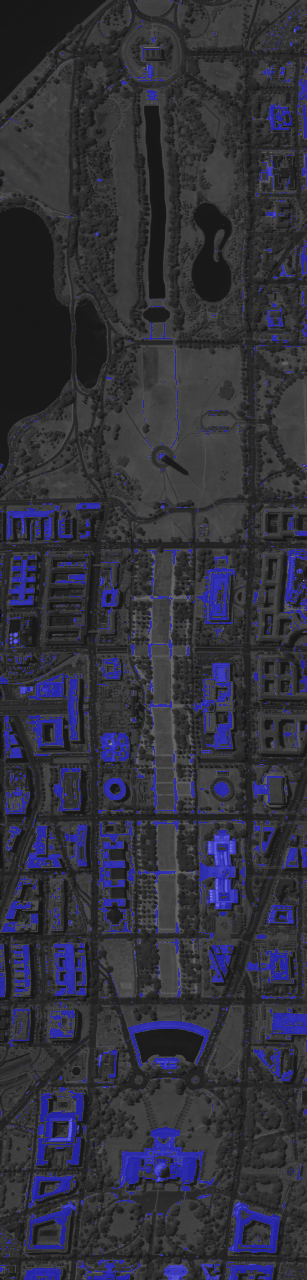
\includegraphics[width=0.8cm,height=3.2cm]{data/DC/13.png}};
                \node[below=0.1] at (11.south) {\textbf{11}};
                \draw[thick,->] (2,-3.2) .. controls (2.5,-3.2) .. (2.5,-4.4);
                \node[inner sep=0pt] (12) at (2.5,-6)
                    {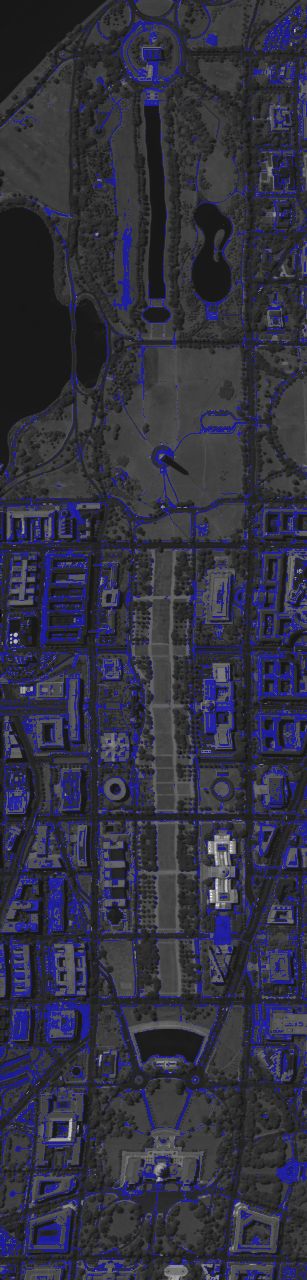
\includegraphics[width=0.8cm,height=3.2cm]{data/DC/14.png}};
                \node[below=0.1] at (12.south) {\textbf{12}};
            \node[below=0.1] at (5.south) {\textbf{5}};
            \draw[thick,->] (3.4,-1.2) .. controls (4.4,-1.2) .. (4.4,-2.4);
            \node[inner sep=0pt] (6) at (4.4,-4)
                {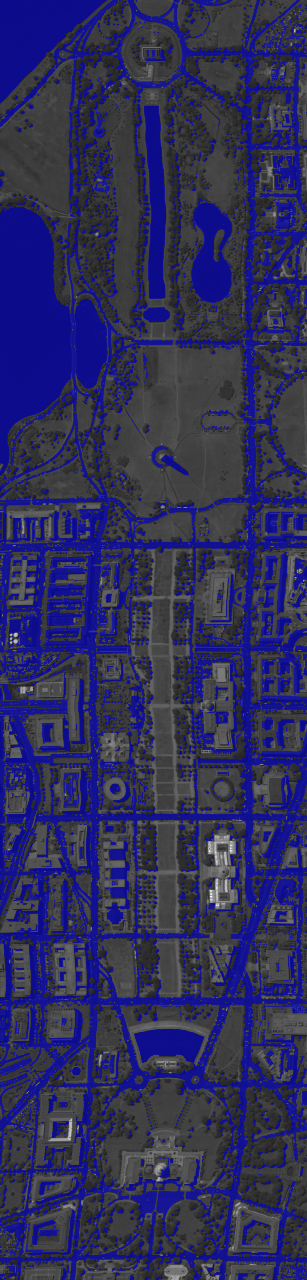
\includegraphics[width=0.8cm,height=3.2cm]{data/DC/5.png}};
                \node[draw, text=orange, fill=white] at (4.4,-4) {water/roads};
            \node[below=0.1] at (6.south) {\textbf{6}};
        \node[below=0.1] at (2.south) {\textbf{2}};
    \node[below=0.1] at (original.south) {\textbf{0}};
\end{tikzpicture}
}